\documentclass[a4paper,12pt]{article}
\usepackage{nameref}
\usepackage{grffile}
\usepackage{graphicx}
\usepackage[strings]{underscore}
\usepackage{verbatim}
\usepackage{wrapfig}
\usepackage{lastpage}
\usepackage{longtable}

\begin{comment}
#
# =====================================================
# $
# $
# $
# $
# $
# =====================================================
#
\end{comment}

\newenvironment{narrow}[2]{
  \begin{list}{}{
    \setlength{\leftmargin}{#1}
    \setlength{\rightmargin}{#2}
    \setlength{\listparindent}{\parindent}
    \setlength{\itemindent}{\parindent}
    \setlength{\parsep}{\parskip}
  }
  \item[]
}{\end{list}}

\title{Next Generation Sequencing report}
\author{\small Genome Analysis Facility (GAF), Genomics Coordination Centre (GCC)\\
\small University Medical Centre Groningen}

\begin{document}
\maketitle
\thispagestyle{empty}
\vspace{40mm}

\begin{table}[h]
	\centering
	\begin{tabular}{l l}
		\hline
		\multicolumn{2}{l}{\textbf{Report}} \\
		Created on & \today \\
		Number of pages & \pageref{LastPage} \\ \\
		Generated by & MOLGENIS Compute \\
		\\
		\multicolumn{2}{l}{\textbf{Project}} \\
		Project name & projectName \\
		Number of samples & 1 \\
		\\
		\multicolumn{2}{l}{\textbf{Customer}} \\
		Principal investigator & me@molgenis.org \\
		\\
		\multicolumn{2}{l}{\textbf{Contact}} \\
		Name & Cleo C. van Diemen \\
		E-mail & c.c.van.diemen@umcg.nl \\
		\hline
	\end{tabular}
\end{table}

\clearpage
\tableofcontents

\clearpage
\section*{Introduction}
\addcontentsline{toc}{section}{Introduction}
This report describes a series of statistics about your sequencing data. Together with this report youll receive a SNP-list. If you, in addition, also want the raw data, then please notify us via e-mail. In any case well delete the raw data, three months after \today.

\clearpage
\section*{Project analysis results}
\addcontentsline{toc}{section}{Project analysis results}

\subsection*{Overview statistics}
\addcontentsline{toc}{subsection}{Overview statistics}
\label{subsect:overviewstatistics}
% statistics table
\begin{table}[h!]
 \caption{Overview statistics}
 \begin{narrow}{-1in}{-1in}
 \centering
\begin{tabular}{l l} 
  \hline 
  Samples$^{(1)}$ & externalSampleID \\ 
  Genome size (bp)$^{(2)}$ & 100 \\ 
  Bait size (bp)$^{(3)}$ & 100 \\ 
  Target size (bp)$^{(4)}$ & 100 \\ 
  Total number of reads$^{(5)}$ & 20 \\ 
  On target bases (Mb) & 0.00017 \\ 
  Aligned bases (Mb)$^{(6)}$ & 0.00017 \\ 
  Mean bait coverage$^{(7)}$ & 1.7 \\ 
  Mean target coverage$^{(8)}$ & 1.7 \\ 
  Fraction bp on bait & 0.85 \\ 
  Fraction bp near bait$^{(9)}$ & 0 \\ 
  Fraction bp off bait & 0 \\ 
  Fraction bp not aligned & 0.055556 \\ 
  Capture specificity$^{(10)}$ & 1 \\ 
  Fraction target covered $\ge$ 2x$^{(11)}$ & 0.45 \\ 
  Fraction target covered $\ge$ 10x$^{(12)}$ & 0 \\ 
  Fraction target covered $\ge$ 20x$^{(13)}$ & 0 \\ 
  Fraction target covered $\ge$ 30x$^{(14)}$ & 0 \\ 
  Fraction usable bases on target$^{(15)}$ & 0.85 \\ 
  Mean read length$^{(16)}$ & 10 \\ 
  Strand balance$^{(17)}$ & 1 \\ 
  Median insert size$^{(18)}$ & 20 \\ 
  Mean insert size$^{(19)}$ & 20 \\ 
  Standard deviation insert size$^{(20)}$ & 0 \\ 
  Number of SNPs for concordance & 2185 \\ 
  Concordance$^{(21)}$ & 0.9997 \\ 
\hline 
\end{tabular}\end{narrow}
 \end{table}



\begin{minipage}{\textwidth}
	Name of the bait set(s) used in the hybrid selection for this project:\\
	\textbf{\input{/Users/mdijkstra/Documents/work/git/molgenis_apps/modules/compute/demo/demoWorkflow/root/groups/gaf/projects/projectName/run00/qc/projectbaitset.txt}}
\end{minipage}

\clearpage
\subsection*{Description statistics table}
\addcontentsline{toc}{subsection}{Description statistics table}
\begin{table}[h!]
	\centering
	\begin{tabular}{r p{12cm}}
		$^{(1)}$ & External sample name\\ 
 $^{(2)}$ & Number of bases in the reference genome used for alignment\\ 
 $^{(3)}$ & Number of bases which have one or more baits on top of them\\ 
 $^{(4)}$ & Unique number of target bases in the experiment where target is usually exons etc\\ 
 $^{(5)}$ & Total number of reads including all PF and non-PF reads\\ 
 $^{(6)}$ & Number of bases in the PF aligned reads that are aligned to the reference genome. Accounts for clipping and gaps (=indels?)\\ 
 $^{(7)}$ & Mean coverage of all baits\\ 
 $^{(8)}$ & Mean coverage of targets with coverage $\ge$ 2\\ 
 $^{(9)}$ & Fraction bp near bait (+/- 250 bp)\\ 
 $^{(10)}$ & Capture specificity; 1 - fraction bases that is off bait\\ 
 $^{(11)}$ & Percentage of ALL target bases with coverage $\ge$ 2\\ 
 $^{(12)}$ & Percentage of ALL target bases with coverage $\ge$ 10\\ 
 $^{(13)}$ & Percentage of ALL target bases with coverage $\ge$ 20\\ 
 $^{(14)}$ & Percentage of ALL target bases with coverage $\ge$ 30\\ 
 $^{(15)}$ & Fraction of aligned, deduplicated, on-target bases out of the PF bases available\\ 
 $^{(16)}$ & Mean read length of the set of reads examined\\ 
 $^{(17)}$ & Number of PF reads aligned to the positive strand of the genome divided by the number of PF reads aligned to the genome\\ 
 $^{(18)}$ & Median of the insert sizes, where insert refers to the base pairs between the adapters.\\ 
 $^{(19)}$ & Mean of the insert sizes, where insert refers to the base pairs between the adapters.\\ 
 $^{(20)}$ & Standard deviation of the insert sizes, where insert refers to the base pairs between the adapters.\\ 
 $^{(21)}$ & Fraction of SNPs that are concordant between array and NGS\\ 
 

	\end{tabular}
\end{table}

\clearpage
\subsection*{Capturing}
\addcontentsline{toc}{subsection}{Capturing}
The following figures show the cumulative depth distribution in the target regions that are located on \emph{chromosome 1}. The fractions of bases that is covered with at least 10x, 20x and 30x are marked with a dot. Please see section "\nameref{subsect:overviewstatistics}" for the full coverage statistics per sample; \emph{i.e.}, in the target regions on \emph{all chromosomes}.
\begin{figure}[ht]\begin{minipage}{0.5\linewidth}\caption{sample \textbf{externalSampleID}}\centering\includegraphics[width=\textwidth]{/Users/mdijkstra/Documents/work/git/molgenis_apps/modules/compute/demo/demoWorkflow/root/tmp/projectName/run00//externalSampleID.coverageplot.pdf}\end{minipage}\hspace{1cm}\end{figure}

\clearpage
\subsection*{Insert size distribution}
\addcontentsline{toc}{subsection}{Insert size distribution}
The following figures show the insert size distribution per sample. Insert refers to the base pairs that are ligated between the adapters.
\begin{figure}[ht]\begin{minipage}{0.5\linewidth}\caption{sample \textbf{externalSampleID}}\centering\includegraphics[width=\textwidth]{/Users/mdijkstra/Documents/work/git/molgenis_apps/modules/compute/demo/demoWorkflow/root/tmp/projectName/run00//externalSampleID.insertsizemetrics.pdf}\end{minipage}\hspace{1cm}\end{figure}

%\clearpage
%\subsection*{Demultiplex statistics}
%\addcontentsline{toc}{subsection}{Demultiplex statistics}
%Under construction...
%displaystats(demultiplexstats)

%\clearpage
%\subsection*{GC metrics}
%\addcontentsline{toc}{subsection}{GC metrics}
%The following figures show the GC-content distribution per sample.
%\begin{figure}[ht]\begin{minipage}{0.5\linewidth}\caption{sample \textbf{externalSampleID}}\centering\includegraphics[width=\textwidth]{/Users/mdijkstra/Documents/work/git/molgenis_apps/modules/compute/demo/demoWorkflow/root/tmp/projectName/run00//externalSampleID.gcbiasmetrics.pdf}\end{minipage}\hspace{1cm}\end{figure}

%\clearpage
%\subsection*{SNP statistics}
%\addcontentsline{toc}{subsection}{SNP statistics}
%The tables with caption Functional type, Functional class and Functional impact, classify the SNPs, based on Ensembl, build 37.64.
%\input{/Users/mdijkstra/Documents/work/git/molgenis_apps/modules/compute/demo/demoWorkflow/root/tmp/projectName/run00//projectName.snps.final.type.tex}
%\input{/Users/mdijkstra/Documents/work/git/molgenis_apps/modules/compute/demo/demoWorkflow/root/tmp/projectName/run00//projectName.snps.final.class.tex}
%\input{/Users/mdijkstra/Documents/work/git/molgenis_apps/modules/compute/demo/demoWorkflow/root/tmp/projectName/run00//projectName.snps.final.impact.tex}

\clearpage
\subsection*{Duplication rates}
\addcontentsline{toc}{subsection}{Duplication rates}
\input{/Users/mdijkstra/Documents/work/git/molgenis_apps/modules/compute/demo/demoWorkflow/root/groups/gaf/projects/projectName/run00/qc/dedupmetrics.txt}

\clearpage
\section*{Appendix 1: SNP-list}
\addcontentsline{toc}{section}{Appendix 1: SNP-list}
The table below explains your SNP-list. The variables that are marked with * or **, are explained in more detail online:\
*snpEff: http://snpeff.sourceforge.net/faq.html\#What_effects_are_predicted? **phred: http://en.wikipedia.org/wiki/Phred_quality_score

\begin{center}
	\begin{longtable}{p{5cm} p{8cm}}
	\caption[SNP-description]{SNP description.}\label{grid_mlmmh} \\

	\hline \multicolumn{1}{l}{\textbf{Name}} & \multicolumn{1}{l}{\textbf{Description}} \\
	\endfirsthead

	\multicolumn{2}{c}%
	{{\bfseries \tablename\ \thetable{} -- continued from previous page}} \\
	\hline \textbf{Name} & \textbf{Description} \\
	\endhead

	\hline \multicolumn{2}{|r|}{{Continued on next page}} \\ \hline
	\endfoot

	\hline \hline
	\endlastfoot

	\tt{Chromosome} & Chromosome number \\
	\tt{Position} & Position on reference genome \\
	\tt{dbSNPid} & dbSNP ID, rs-number \\
	\tt{Reference allele} & Reference allele \\
	\tt{Alternative allele} & Alternative allele \\
	\tt{Quality} & Quality score, phred** scaled \\
	\tt{Filter} & Passed filter when value is PASS \\
	\tt{Allele balance} & Allele balance for hets (ref/(ref+alt)) \\
	\tt{Allele count} & Allele count in genotypes, for each alternative (ALT) allele \\
	\tt{Allele number} & Total number of alleles in called genotypes \\
	\tt{BaseCounts A C G T} & Number of called bases in the order of A,C,G,T \\
	\tt{Depth} & The number of bases covering this site, also known as coverage \\
	\tt{GC content} & GC content within 20 bp +/- the variant site \\
	\tt{Mapping quality} & Mapping quality, phred scaled \\
	\tt{Quality by depth} & Variant confidence/quality by depth \\
	\tt{Strand bias} & Strand bias \\
	\tt{snpEff amino acid change*} & Amino acid change \\
	\tt{snpEff codon change*} & Codon change: old codon/new codon \\
	\tt{snpEff effect*} & Predicted effect of the variant, for a list of all effects see * \\
	\tt{snpEff exon ID*} & Chromosomal position depicted as: exon chromosomenumber start end \\
	\tt{snpEff functional class*} & Functional class, has one of these values; NONE, SILENT, MISSENSE, NONSENSE \\
	\tt{snpEff gene biotype*} & Biotype, as reported by ENSEMBL \\
	\tt{snpEff gene name*} & Gene name \\
	\tt{snpEff impact*} & Effect impact, can be one of these values; High, Moderate, Low, Modifier \\
	\tt{snpEff transcript ID*} & Transcript ID, as reported by ENSEMBL \\
	\tt{Sample} & Sample ID \\
	\tt{dbSNP132 allele frequency} & Allele frequency of the variant as known in dbSNP \\
	\tt{1KG $>5~\%$ MAF in >1 populations} & $>5$\% Minor Allele Frequency in one of the 1000 genomes populations (1=true, 0=false) \\
	\tt{1KG $>5~\%$ MAF in each and all populations} & $>5$\% Minor Allele Frequency in all 1000 genomes populations (1=true, 0=false) \\
	\tt{Discovered in 1KG production phase} & Variant is discovered in 1000 genomes production phase (1=true, 0=false) \\
	\tt{Discovered in 1KG pilot1} & Variant is discovered in 1000 genomes pilot phase (1=true, 0=false) \\
	\tt{Discovered in 1KG all pilots} & Variant is discovered in all 1000 genomes pilots (phase 1,2,3) (1=true, 0=false) \\
	\tt{Discovered in 1KG and validated by second method} & Variant is discovered in 1000 genomes and validated using a secondary method (1=true, 0=false) \\
	\tt{First included in dbSNP release} & dbSNP version in which this variant was reported for the first time \\
	\tt{Genotype} & Genotype for the variant, where 0=reference and 1=alternative \\	\end{longtable}
\end{center}

\clearpage
\section*{Appendix 2: Genome Analysis Facility Pipeline}
\addcontentsline{toc}{section}{Appendix 2: Genome Analysis Facility Pipeline}
\subsection*{Exome sequencing}
\addcontentsline{toc}{subsection}{Exome sequencing}
\begin{wrapfigure}{r}{0.5\textwidth}
	\begin{center}
		\includegraphics[width=.5\textwidth]{/Users/mdijkstra/Documents/work/git/molgenis_apps/modules/compute/demo/demoWorkflow/root/tools/getStatistics_20121127/GAFpipeline.png}
	\end{center}
	\caption{Workflow in the lab}
	\label{fig:wet}
\end{wrapfigure}
Figure \ref{fig:wet} illustrated the basic experimental process of exome capture sequencing. The Genomic DNA sample was randomly fragmented using Nebulisation. Then barcoded adapters were ligated to both ends of the resulting fragments, according the standard New England Biolabs protocol. Fragments with an insert size of 220 bp on average were excised using the Caliper XT gel system and the extracted DNA was amplified with PCR.

The quality of the product was verified on the BioRad Experion instrument. If the quality of the product meets the criteria, the product is multiplexed in an equimolar pool of 4 simular products. This pool is hybridized to the Agilent SureSelect All exon V2, according the provided protocol. After amplification of the enriched products with PCR the quality of the products is verified on the BioRad Experion instrument and Paired End sequenced on the HiSeq2000 with 100 bp reads. Image Files were processed using standard Illumina basecalling software and the generated reads are ready for downstream processing after demultiplexing.

\clearpage
\section*{Appendix 3: Bioinformatics pipeline}
\addcontentsline{toc}{section}{Appendix 3: Bioinformatics pipeline}
Your samples have been anlayzed with bioinformatics pipeline shown in Figure \ref{fig:dry}.
\begin{figure}[h]
	\caption{Bioinformatics pipeline. The ovals describe the steps in the pipeline. The arrows indicate the work flow of data between the steps.}
	\begin{center}
		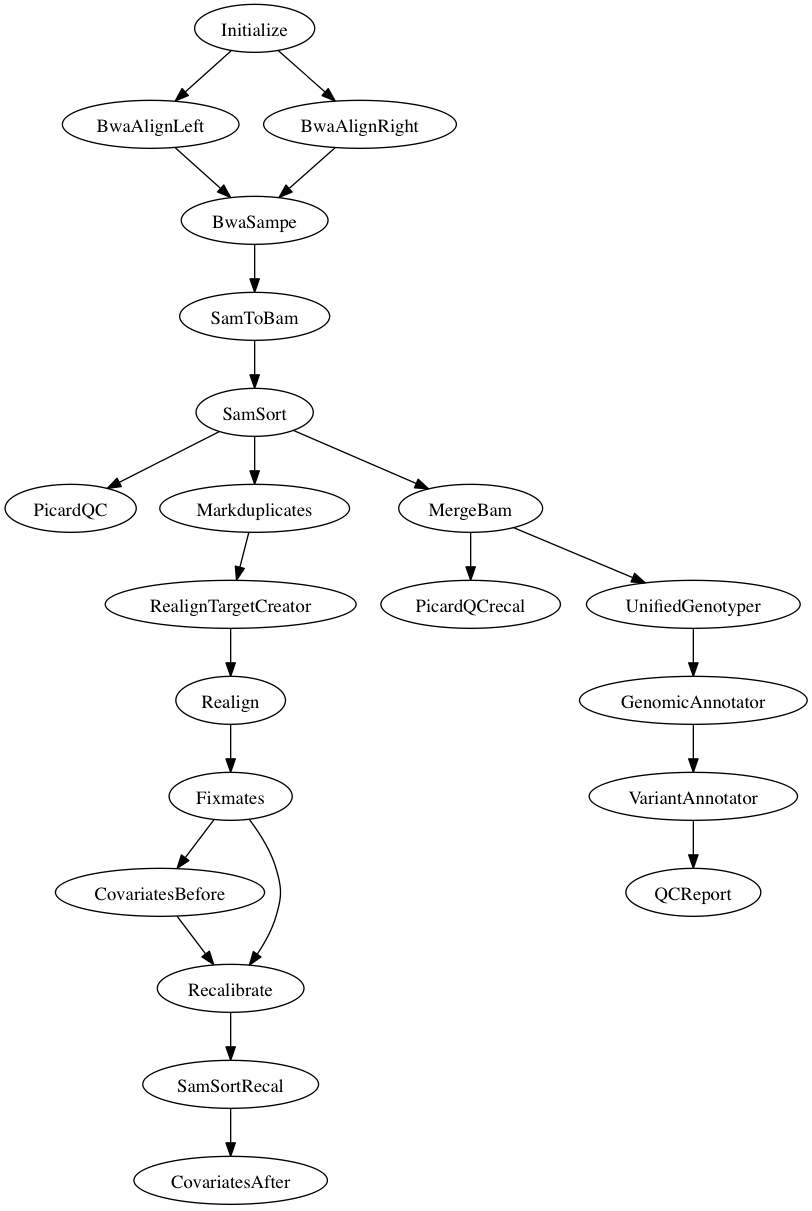
\includegraphics[width=.9\textwidth]{/Users/mdijkstra/Documents/work/git/molgenis_apps/modules/compute/demo/demoWorkflow/root/groups/gaf/projects/projectName/run00/qc/projectName_workflow.png}
	\end{center}
	\label{fig:dry}
\end{figure}
\end{document}
